\chapter{State of the Art}

\section{Introduction}

Information Security is one of the key issues that slows down the development of cloud computing and its feature of complications with data privacy and protection continue to hinder taking the market\cite{Subashini2011}. Although the cloud storage services potentially offer several security advantages with their standardized accessing interfaces and benefits of scale (i.e., the same investment of security infrastructures on centralized server sets would provide better capability with regard to issues like data filtering, update management and deployment of information security policies) and agility of reactions to attacking events or other security-threatening behaviors. However, in some other ways, due to its essence of the multi-tenancy model\cite{Dillon2010}, problems are caused by sharing physical storage resources with other users. Also its nature of SaaS implies merely the accessing and auditing interfaces are open to users makes the hidden internal mechanism not trustworthy to users. Furthermore, security approaches towards cloud storage must consider interactions and mutual effects among multiple network objects (e.g., other applications or users)\cite{Ou2005} that lead to the invalidation or rejection of traditional local secure storage methods. Modern security technologies and some mainstream cloud storage security solutions in particular are considered as referable potential solutions to this problem. Their features, impacts and also reasons why some of these security approaches are not appropriate in certain application scenario will be discussed in this chapter.

\section{Cryptography}

“Cryptography provided secrecy for information sent over channels where eavesdropping and message interception was possible”\cite{Rob1982}. In order to conceal sensitive contents, cryptography is always exploited on plain text in the storage media concerning not only those intelligible contents but also metadata that might be utilized for deducing the corresponding contents.

\subsection{User-level Cryptography}

A typical way of encrypting the file or data is through some encryption tools, such as enigma under FreeBSD, crypt in UNIX or applications with encryption modules embedded. The basic goal of information concealing achieved in this way if used properly. However, none of them is entirely satisfying in the matter of security, generality and availability\cite{Zhang2010}. Manual errors like forgetting to delete the plain text file after encryption or inappropriate key management will make results far from expectation. As a conclusion, if encryption is too close to the user level, the high frequency of human interaction caused errors is not worth the cumber for practical and everyday usage\cite{Laboratories1993}.

\subsection{System-level Cryptography}

Generally to avoid the manual flaws of user level encryption, the cryptographic related modules should be designed to serve as infrastructures of the system. The key of designing this system is mainly about specifying the component to be cryptographically protected in accordance with priority level. Storage and communication risks are most urgent factors to be concerned about.

Physical media like hard drives could be well protected by customizing the hardware design or additional firmware functionalities. Disk controllers could be used for encrypting entire disks or individually ciphering file blocks with a specified key. In this way the procedure of encryption is completely transparent as long as the key is determined to the hardware\cite{Laboratories1993}. It seems to be an ideal alternative of user-level cryptography but the problem happens when performing data management like sharing or backup. Data sharing would not be done until the encryption key exchange has been made via unreliable medium. Playing backup of a disk without encrypting raw contents is equivalent to exposing a decrypted version of ciphers while applying same encryption mechanism gives rise to not only extra expense of backup procedure but other unreliability concerns. For example, backup is periodically played to ensure the availability by creating data redundancy. However, an extra cryptography application will make the availability of cryptography modules a necessary condition prior to the availability of content backup itself, which changes the essence of backup drastically.

Moreover, such mechanism would not protect data commuting with the disk so that it is not sufficient to secure data in remote physical storage entities. Encrypted network connections between storage entities could be a solution for securing the data exchange. The cryptography could be utilized in the form of end-to-end encryption communication protocol and cryptographic authentication\cite{Laboratories1993}. However, some specialized hardware might be required and these extra cryptographic operations will doubtlessly cause a significant penalty of network performance.

\section{Secure Storage in the Cloud}

File systems on the cloud, due to their web application circumstance, lead to extra security concerns in comparison to local file system. Except for enhancement of its service availability, features like constant monitoring and auditing mechanism will be well redesigned and integrated into the system to achieve better security performance\cite{Ghemawat2003}. Most service providers offer access control mechanism as a basic security issue. Some service carriers (e.g., Dropbox) use a combination of identity based access control and encrypted data storage while others (e.g., Google Drive) just stick to concentrating on better access control, auditing performance and revolutionary redesign of the traditional file system, Google File System for instance. Also, certain modern solution like two-step verification which refers authentication security to additional verification steps via text, voice call or other similar approaches. It adds an extra layer for secure storage thanks to carriers’ multi-platform features.

\subsection{Security in Dropbox}

Dropbox uses Amazon's Simple Storage Service (S3) as storage infrastructure. All files stored online by Dropbox are encrypted during transmission and before storage with Secure Sockets Layer (SSL) and AES-256 bit encryption respectively\cite{Dropbox2013}. Amazon S3 does not encrypt data before storage but a service named Server Side Encryption (SSE) is provided for users to encrypt files and perform key management on the cloud.

\subsection{Security in Google Drive}

Without using any local encryption on the physical storage infrastructure, Google improves its file system dramatically about the access control and auditing. In Google File System, there are some innovative specific fields as part of file metadata for multi-user management and data sharing. For example, rather than generating physical replicas of file or file relocation record, the field ``exportLinks'' allows data sharing by generating a sharing URL which is irreversible and ready to be published. Another field ``writersCanShare'' indicates the writer’s permission of sharing the file with others, which actually controls the permission leakage.

Google Drive also offers another access control mechanism called authorization scope. Authentication scopes imply the permissions users are required to authorize for the following operations. For example, when requiring for authorization with CGI: /auth/drive.readonly indicates that a positive authentication result will allow read-only access to file metadata and file content.

\subsection{Storage Security Risks in the Cloud}

Privacy concerns for some internal reasons always exists as long as the content is stored in plain text on the cloud or encrypted with a key that is known to someone who conducts the encryption. Dropbox has been criticized for storing authentication information on disk in plain text. It actually indicates that Dropbox's terms of service are contradicted to its privacy implementation although the company claims that employees of Dropbox are not able to access user’s files or profiles\cite{Icaza2011}. On the contrary, employees of Dropbox can effortlessly hack the system and access user’s data unconsciously\cite{Dhillon2001}. This kind of attacks cannot be protected by traditional security technologies as long as it is technically possible\cite{Yao2010}.

External attackers would also try to hack the storage service provider’s system to access to stored data and such attacking could be prevented by traditional approaches\cite{Uppalli2003}. Undoubtedly, it will raise the data security risk if stored plain texts are exposed once the system has been exploited. Given the fact that these day and night services with considerable potential profit are more attractive to attackers, they are essentially more information secure risky. Some services claim that the stored data is all well encrypted but tragedy happens when key management are played in the same bucket and easily to be discovered by hackers.

Anyway, storage on the cloud in plain text, no matter how unbeatable the security design and implementation are, is highly risky no matter it is facing an internal or external attack. Customer data is uncontrolled and could be leaked to unaccredited parties potentially in this way\cite{Uppalli2003}.

\section{Searchable Symmetric Encryption}

The security of encrypted data storage, assuming the private key could be kept properly and confidentially, could be guaranteed. However, there could be an availability performance penalty that routine private key encryptions might prevent searching over encrypted data. Users would lose the ability to selectively locate fragments of expected data at the same time\cite{Kamara2010}\cite{Xiaodong2000}. Searchable symmetric encryption (SSE) allows user to use the third party storage service of its data, meanwhile keeping the capacity of selective searching over data pools\cite{Curtmola2006}.

The system prototype was described as a possible architecture for a cryptographic storage service in the paper from Microsoft\cite{Curtmola2006}. The system was composed of three parts: a data processor (DP), a data verifier (DV) and a token generator (TG). The data processor handles data prior to being sent to the cloud; Data verifier verifies if the data in the cloud has been modified without authorization based on auditing information; Token generator generates tokens that grant the permissions to the cloud storage provider and enables it to get segments of expected data on customer. Additionally, a credential generator who works based on certain access control mechanism is implemented. It works by issuing credentials to the various parties in the system which will enable them to decrypt encrypted files according to the policy.

The key features of a cryptography based storage service let customers take control of their data. Its security properties are derived from cryptography, a trusted issue but not those unreliable human factors like legislation or physical security. The advantage with regard to security make the data is always encrypted and data integrity can be audited any time so that security attacking poses little, or say, no risk for the customer\cite{Kamara2010}. Furthermore, the utilization of symmetric searchable encryption, which leaves the indexes available but sensitive contents encrypted, improves the availability of encryption based security storage.

\begin{figure}[h]
        \centering
        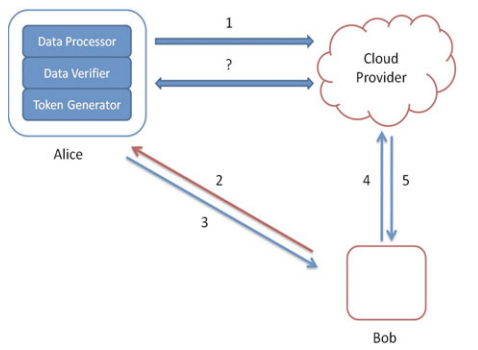
\includegraphics[width=0.6\textwidth]{figures/Customer_Architecture.png}
        \caption[Customer Architecture] {Customer Architecture\cite{Kamara2010}}
\end{figure}

The whole process illustrated in this paper is expressed as follows:
\begin{enumerate}
  \item 
  Alice’s data processor prepares the data (encrypted with symmetric searchable encryption) before sending it to the cloud.
  \item 
  Bob asks Alice for permission to search for a keyword.
  \item 
  Alice’s token and credential generators send a token for the keyword and a credential back to Bob.
  \item 
  Bob sends the token to the cloud.
  \item 
  The cloud uses the token to find the appropriate encrypted documents and returns them to Bob.
  \item 
  At any point in time, Alice’s data verifier can verify the integrity of the data.
\end{enumerate}

\section{FileMap}

“FileMap is a file-based map-reduce system for data-parallel computation”\cite{Mfisk2013}. It is designed and implemented around several application scenarios like file-based and data replication. Its idea of data replication mechanism which is similar to RAID4 or RAID5 means the file is split in the physical separated media and stored. Files could be split into segments and stored in different entities which are both logically or physically separated, or a combination of them. For example, to perform secure cloud storage in logical separated entities, certain file could be fragmented into n segments and stored in one provider’s cloud storage service with n identities (i.e., n segments stored in n accounts of Dropbox respectively). While storing files in physical separated entities, as same as the first scenario, files also have to be divided into n segments but the difference is storing them via different cloud storage providers’ services (i.e., n segments stored in Google Drive, Dropbox and SkyDrive separately). Given the fact that some providers providing encrypted storage service like Dropbox, a pseudo searchable encrypted cloud storage prototype with could be made by:
\begin{enumerate}
  \item 
  Regenerate the file and adding indexes information in the metadata and fragment it into index and content segments.
  \item 
  Store the index segments in plain text stored cloud storage service but with better access control mechanism deployed like Google Drive.
  \item
  Store the rest n content segments in n accounts of encrypted cloud storage service like Dropbox.
\end{enumerate}
